%%%%%%%%%%%%%%%%%%%%%%%%%%%%%%%%%%%%%%%%%
% University/School Laboratory Report
% LaTeX Template
% Version 3.1 (25/3/14)
%
% This template has been downloaded from:
% http://www.LaTeXTemplates.com
%
% Original author:
% Linux and Unix Users Group at Virginia Tech Wiki 
% (https://vtluug.org/wiki/Example_LaTeX_chem_lab_report)
%
% License:
% CC BY-NC-SA 3.0 (http://creativecommons.org/licenses/by-nc-sa/3.0/)
%
%%%%%%%%%%%%%%%%%%%%%%%%%%%%%%%%%%%%%%%%%

%----------------------------------------------------------------------------------------
%	PACKAGES AND DOCUMENT CONFIGURATIONS
%----------------------------------------------------------------------------------------

%\documentclass[12pt]{article}
\documentclass[14pt]{extarticle}

\usepackage{setspace} % For set space
\usepackage{algorithm} % For pseudo code
\usepackage[noend]{algpseudocode}
\usepackage{siunitx} % Provides the \SI{}{} and \si{} command for typesetting SI units
\usepackage{graphicx} % Required for the inclusion of images
\usepackage{amsmath} % Required for some math elements 
\usepackage{cite} % For citation

\setlength\parindent{0pt} % Removes all indentation from paragraphs
\setlength{\parskip}{0.5em}

\renewcommand{\labelenumi}{\alph{enumi}.} % Make numbering in the enumerate environment by letter rather than number (e.g. section 6)
\renewcommand{\baselinestretch}{1.5}
%\usepackage{times} % Uncomment to use the Times New Roman font

%----------------------------------------------------------------------------------------
%	DOCUMENT INFORMATION
%----------------------------------------------------------------------------------------

\title{\large Multiple AI Competition in Self Developed Game \\ Term 1 Report \\ ESTR4998/4999} % Title

\date{\today} % Date for the report

\begin{document}


\maketitle % Insert the title, author and date

\begin{center}
\begin{tabular}{l r}
Partners: & XIAO Tianyi \\ % Partner names
& LUO Lu \\
Instructor: & Prof. Andrej Bogdanov % Instructor/supervisor
\end{tabular}
\end{center}
\newpage


%----------------------------------------------------------------------------------------
%	SECTION 1
%----------------------------------------------------------------------------------------

\begin{abstract}
	Abstract text
\end{abstract}
 
%----------------------------------------------------------------------------------------
%	SECTION 2
%----------------------------------------------------------------------------------------

\section{Background}

\subsection{Related Works}
As the development of science technology, the game also evolves from the ancient chess game to the fantastic AAA video games nowadays. And with the development of artificial intelligence, bulding an agent to play a game is always a popular and interesting topic. Up to now, there are many research on playing game with nerual netwrok, like AlphaGO(Silver et al), playing Atari game(Mnih et al), and playing Dota2(Berner et al).\\\\
Inspired by previous works, we found that Reinforcement Learning is widely used in game agent training. Therefore, we decide to build reinforcement learning model in our project. Also, the game to be played by AI will be developed by ourselves, which is a soccer game.\\\\
Our goal is to build an agent which is able to play the game with certain strategy. And an agent which can beat normal human being would be satisfactory. What's more, by adjusting configuration of the game, we wish to know if our agents could cooperate with their teammates in the multiple players mode(like 2v2 or 5v5).

\subsection{TensorFlow}
TensorFlow is a free and open-source software library for machine learning, which was first realeased in 2017. TensorFlow is commonly used in deep neural networks. And in this project, keras, which works as the interface for TensorFlow, is used to build our nerual network.

\subsection{Pygame}
Pygame is a set of Python modules for making computer games, which was first realeased in 2020. Though Pygame may not support fantastic 3D game, however, it is simple and easy to learn and use.\\\\
Additionally, considering the training process of AI, a game platform based on Python would be more suitable than other main stream game development platforms nowadays, like Unity or Unreal Engine 4. That is the reason why we choose Pygame as our game development platform.


%----------------------------------------------------------------------------------------
%	SECTION 3
%----------------------------------------------------------------------------------------

\section{Introduction}

\subsection{Agents Design}
\subsubsection{Reinforcement learning}

Reinforce learning is an area of machine learning and artificial intelligence, which concerns about how agents will take actions to achieve the best outcome in a environment. Unlike the supervised learning, reinforce learning does not need labelled data, and it focuses on exploration and exploitation. Agents can take randomly actions and receive correspond rewards to explore current environment. Agents can also make decisions by exploiting the current knowledge which comes from the exploration.

A basic reinforcement is modeled as Markov Decision Process, and a MDP consists of 4 parts:
\begin{itemize}
    \item [1)] A finite set of environment and agent states, named $S$
    \item [2)] A finite set of action of agents, named $A$
    \item [3)] Transition functions $T$
    \item [4)] Reward function $R$
\end{itemize}
Reinforcement learning is widely used in many area, including animal psychology, game theory and create bots for video games. In our project, we will implement at least two kinds of reinforcement learning  model: $Q$-learning and Deep $Q$-Network(DQN), discuss the advantage and disadvantage of each of them, and compare the different of them about their response when we change the rewards function or the configuration of our game.

\subsubsection*{\small Implementation detail of Reinforcement learning}

Most of the reinforcement learning method are model-free, which means the algorithm does not require the prior  known about the transition and reward functions and the agents need to estimate the models by interacting with the black box, environment.

The pseudo code of reinforcement learning is shown in Algorithm 1.

\begin{algorithm}
    \caption{Reinforcement Learning (Zoph et al, 28) }\label{euclid}
    \begin{algorithmic}[1]
    \State Initialize $\tilde{T}, \tilde{R}, \tilde{Q} \ and/or\  \tilde{V}$
    \For{each episode}
        \State $s \in S$ is initialized as the starting state
        \State $t := 0$
        \Repeat
            \State choose an action $a \in A(s)$
            \State perform action $a$
            \State observe the new state $s'$ and received reward $r$
            \State update $\tilde{T}, \tilde{R}, \tilde{Q} \ and/or\  \tilde{V}$
            \State using the experience $\left\langle s,a,r,s'\right\rangle $
            \State $s := s'$
            \State $t := t + 1$
        \Until $s'$ is a goal state or $t$ reaches the limitation
    \EndFor
    \end{algorithmic}
\end{algorithm}

In this pseudo code, $\tilde{T}$, $\tilde{R}$, $\tilde{Q}$ and $\tilde{V}$ are the estimates of the agent, and they should be initialized before the training section. For each episode, we reset the environment, and initialize it to the starting state. Then the agents will repeatedly choose an action randomly or based on the knowledge, observe the return of the environment and update the estimates. For some environment, there are some goal states, and the episode will stop when one of the goal state is reached. Notice that goal states are terminal states,not the best or winning states.

\subsubsection{$Q$-learning}

$Q$-learning is one of the most basic and popular temporal difference learning method to estimate Q-value function(Zoph et al, 31). Temporal difference method use estimates of other value to learn their value estimates, and the update rule of TD method is: 

$$V_{k+1}(s) = V_{k}(s) + \alpha(r + \gamma V_k(s') - V_k(s))$$ 

In this equation, $k$ is the times of iteration, $s$ is the state to be updated, $\alpha$ is the learning rate which should be gradually decreased as iterating, $\gamma$ is the discount factor and $r$ is the received reward.

In Q-learning, the basic idea is similar to the temporal difference learning. The difference is that value estimates $V$ becomes $Q$-value function, and the estimates of other values become the previous agent's $Q$-value function. Therefore, the update rule of $Q$-learning is a variation of TD learning:

$$Q_{k+1}(s_t, a_t) = Q_{k}(s_t, a_t) + \alpha(r_t + \gamma max_{a}Q_k(s_{t+1},a) - Q_k(s_t, a_t))$$

The difference between $Q$-value estimate and the value estimate in TD is that in the same state, the $Q$-value for different actions can be different. The transition function is determined, which means for a state $s_t$ and the agent takes an action $a_t$, the agent will walk to a certain state $s_{t+1}$ and receive reward $r_t$. The discount factor $\gamma$ will determine how much the expected future rewards affect the current estimates. The algorithm will focus more on short-term rewards if the $\gamma$ is set lower. 

The advantage of $Q$-learning is that it's exploration-insensitive, which means we can get the optimal policy as long as the $\alpha$ is set properly and every state-action pairs can be visited infinite times(Zoph et al, 31).

However, the drawback of $Q$-learning is also obvious. We need to store every state-action pairs in the $Q$ table, but the numbers of states and actions are huge in many environments because the dimensions of the state are high. For each pair, we need to visit it adequate times, to update the $Q$-value, which is time-consuming, even impossible. In our project, we will show how this disadvantages affect the performance of $Q$-learning.

\subsubsection*{\small Implementation detail of $Q$-learning}

The pseudo code of $Q$-learning is shown as Algorithm 2.

\begin{algorithm}
    \caption{Reinforcement Learning (Zoph et al, 31) }\label{euclid}
    \begin{algorithmic}[1]
    \Require $\gamma$, $\alpha$
    \State Initialize $Q$ (e.g. $Q(s,a) = 0 \ for \ \forall s \in S, \forall a \in A$)
    \For{each episode}
        \State Modify $\alpha$ and $\gamma$
        \State $s \in S$ is initialized as the starting state
        \Repeat
            \State choose a random action or the best action $a \in A(s)$ based on the exploration strategy.
            \State perform action $a$
            \State observe the new state $s'$ and received reward $r$
            \State \small $Q_{k+1}(s, a) = Q_{k}(s, a) + \alpha(r + \gamma \cdot max_{a \in A(s')}Q_k(s,a') - Q_k(s', a))$
            \State using the experience $\left\langle s,a,r,s'\right\rangle $
            \State $s := s'$
        \Until $s'$ is a goal state or $t$ reaches the limitation
    \EndFor
    \end{algorithmic}
\end{algorithm}


\begin{table}[]
    \begin{center}
        \begin{tabular}{|c|c|c|c|c|}
        \hline
        $Q$-table & a\_1 & a\_2 & ... & a\_n \\ \hline
        s\_1      & 0    & 1    & ... & 0    \\ \hline
        s\_2      & 1    & 0    & ... & 0    \\ \hline
        ...       & ...  & ...  & ... & ...  \\ \hline
        s\_n      & 0    & 0    & ... & 1    \\ \hline
        \end{tabular}
        \caption{$Q$-table}
    \end{center}
\end{table}    


$Q$-learning is a kind of Reinforcement learning, so the main procedure is similar. However, there are some details to be noticed. 

First, the estimates of $Q$-learning is $Q$-table. A $Q$-table will be initialize before the training section. $Q$-table is a table consists of the states of the environment and the action. For example, one possible $Q$-table is similar to Table 1.

Second, in the start of each episode, we may need to decrease the learning rate - $\alpha$, to ensure the $Q$-table can converge finally. We also need to decrease the probability of random action, and the agent will make decisions more based on the knowledge got from exploration.

\subsubsection{Deep $Q$-Network} 

As the previous part mentioned, the performance of $Q$-learning in high dimensional environment is not satisfied. However, the previous tries at using neutral network to represent the action-value function were failed. The reinforcement learning is unstable or even diverge because of the correlations present in the sequence of observation(Mnih et al). 

This problem was finally solved by DeepMind, and the solution is called DQN. DeepMind introduced two techniques to remove the correlations. One is experience replay, inspired from a biological mechanism. By using this technique, the agent will save amount of experiences(state-action-reward-state) in the dataset, called "memory". Then, the algorithm will randomly choice a small batch of experiences from the memory to apply $Q$-learning. There are some advantage to use this strategy compared the traditional $Q$-learning, and one of them is that this strategy can significantly remove the correlation and make the approximator stable.

The second technique is to use two separate networks. One is called target network $Q$, which is cloned from the original network $Q$ every $C$ updates. The target network is used for updating network $Q$, in the right side of update rule. This method can also decrease the correlation and make the algorithm more stable.

\subsubsection*{\small Implementation detail of DQN}

The pseudo code of DQN provided by DeepMind is shown in Algorithm 3.
\begin{algorithm}
    \caption{Deep $Q$-Network(Mnih et al)}\label{euclid}
    \begin{algorithmic}[1]
    \State Setup replay memory $D$ to capacity $N$
    \State Initialize action-value function $Q$ with random weights $\theta$
    \State Initialize target action-value function $\hat{Q}$ with weights $\theta'$
    \For{each episode}
        \State Initialize sequence $s_1 = {x_1}$ and preprocessed sequence $\phi_1 = \phi(s_1)$
        \State $t := 1$
        \Repeat
            \State choose a random action or the best action $a_t \in A(s)$ based on the exploration strategy.
            \State perform action $a_t$
            \State observe the new input $x_{t+1}$ and received reward $r_t$
            \State Set $s_{t+1} = s_t,a_t,x_{t+1}$ and preprocess $\phi_{t+1} = \phi(s_{t+1})$
            \State store the experience $(\phi_t, a_t, r_t, \phi_{t+1})$ in $D$
            \State Sample random minibatch of transitions $(\phi_j, a_j, r_j, \phi_{j+1})$ in $D$
            \State Set $y_j = r_j + \gamma max_{a'} \hat{Q}(\phi_{j+1},a'; \theta')$
            \State Perform a gradient descent step on $(y_j - Q(\phi_j, a_j; \theta))^2$ with respect to the network parameters $\theta$
            \State Every C steps reset $\hat{Q} = Q$ 
        \Until $s'$ is a goal state or $t$ reaches the limitation
    \EndFor
    \end{algorithmic}
\end{algorithm}
%----------------------------------------------------------------------------------------
%	SECTION 4
%----------------------------------------------------------------------------------------

\section{Design}

The design of our FYP is based on two parts, which are the game part and AI part.

\subsection{Game Design}

\subsubsection{Game Mode}
In consideration of the cost of game development, basically the time cost, we decide to implement a game with straightforward structure. For the purpose of AI training, the game should have one clear goal and controllable user inputs, otherwise the workload and cost of the FYP could be hard to measure. Then as the result of teamwork discussion, soccer game is chosen as the game mode.

\subsubsection{Game Rule}
\begin{description}
	\item[Team and players]
	There are two teams (team-0 and team-1) in the game. For each team, ther are N players (1 $\leq$ N $\leq$ 7).
	\item[Goal]
	If a ball pass through the goal of a team, then opposite team would get a score. And in each turn of the game, the team who get most scores will win the game, otherwise it ends in a draw. Therefore, for each team, they should try their best to get more scores and prevent the opposite team to get any score.
	\item[time]
	Every turn of game has a time limit. As soon as it reaches time limit, this turn of game will be forcely over.
\end{description}

\subsubsection{Player Action}
For each player, it can get the ball when it is free, steal the ball when it is catched by another player, and shoot the ball when it is catching the ball.
\begin{description}
	\item[catch]
	When a ball is not catched by any player, any player can try to get the ball. As soon as a player touch the ball, the player will get the ball.
	\item[Steal]
	When a ball is catched by a player, other players can steal the ball from player. As long as another player touch the player with ball, the ball would be stolen. However, after a player just get the ball, there will be a short invincible period. Only after the invincible period, can other players steal the ball.
	\item[shoot]
	When a player is catching the ball, the player can shoot the ball away. It can shoot the ball along the eight directions, which are left, right, up, down, upper-left, upper-right, lower-left, lower-right.\\
	And for the player just shoot the ball, it need to wait for a short period to be able to get the ball again.
\end{description}

\subsubsection{Other Details About Game}
\begin{description}
	\item[boundary]
	When the ball reach the boundary, it will bounce back. Players are not able to get out of boundary.
	\item[Initialization and Reset]
	When each turn of game begins, every player would be assigned to an initial position, and ball will be placed in the center of the field. And when any of two teams get a score, the positions of players and ball will also be reset to initial positions.
\end{description}

\subsection{AI Design}
\subsubsection{Objection}
The objection of our project is %todo
Therefore we design 2 kinds of agents in this project, the agent using $Q$-learning and the agent using DQN. The former is simpler, and don't need the use of machine learning. The latter is an artificial intelligence and expected to perform better.
\subsubsection{Structure of Agents}

\begin{description}
	\item[Sensor]
    In some researches, agents are created for existing video game, so the sensors of them are image recognizing CNN which are fed by screenshots of the game. For example, the researchers in DeepMind use CNN to read information from the screenshots of Atari games(Mnih et al).

    However, in our project, the environement are designed for training agents from the very beginning. The agents can directly get the information, including the position of every agents and ball, by using some method. In this way, we simplify the sensor part, and the quality of CNN will not effect the training results which are most concerned.
    
	\item[Initialization and Reset]
    When each turn of game begins, every player would be assigned to an initial position, and ball will be placed in the center of the field. And when any of two teams get a score, the positions of players and ball will also be reset to initial positions.
    
\end{description}



%----------------------------------------------------------------------------------------
%	SECTION 5
%----------------------------------------------------------------------------------------

\section{Implement}

\subsection{Game Implementation}

In our pygame implementation of the soccer game, we build two important classes \textbf{Player} and \textbf{Ball}.

\subsubsection{Player}
The Player class inherits from Sprite, which is a pre-defined class of pygame module. Below are methods of Player.
\begin{description}
	\item[\_\_init\_\_]
	In the \_\_init\_\_ method, we define and initialize the related variavles of a player, assign an id and initial position to the player, and load the image of players.
	\begin{figure}[H]
		\begin{center}
			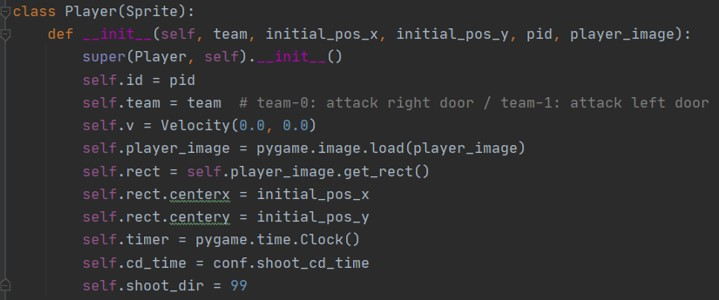
\includegraphics[width=0.9\textwidth]{Player_init}
			\caption{implementation of \_\_init\_\_ in Player}
		\end{center}
	\end{figure}
	\item[input\_handler]
	In the input\_handler, an input array is passed into the method. The input array contains information about user input, including the four moving directions along x and y axes, and if the user want shoot the ball. If no user input on one axis, or two opposite directions (like up and down, or left and right) show up at the same time, the player will not have velocity on that axis. Otherwise, the velocity will be added on the corresponding directions. If the user want to shoot the ball, the related shoot\_dir will be calculated through xy\_to\_dir, and then be dealt with if the ball belongs to this player.
	\begin{figure}[H]
		\begin{center}
			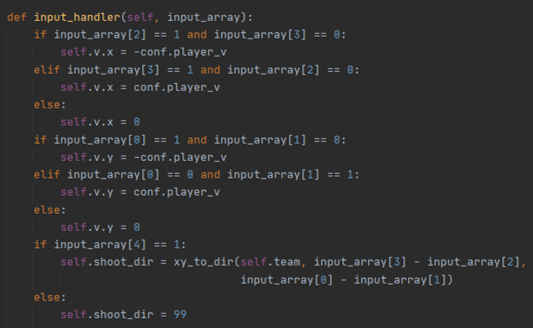
\includegraphics[width=0.9\textwidth]{Player_input}
			\caption{implementation of init\_handler in Player}
		\end{center}
	\end{figure}
	\begin{figure}[H]
	\begin{center}
			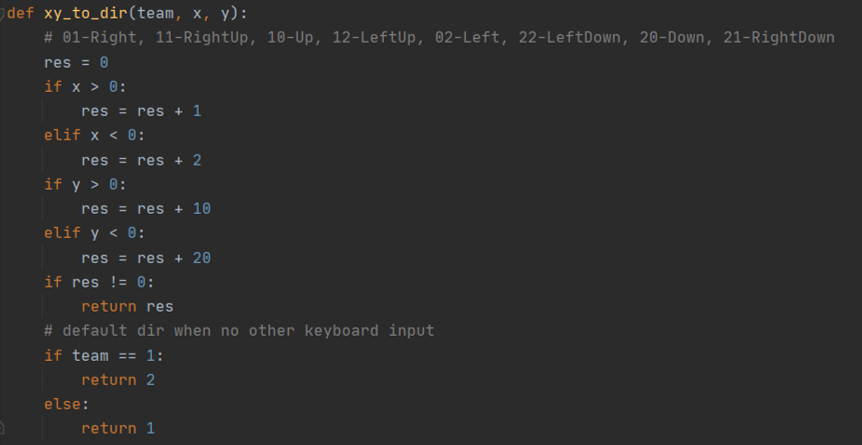
\includegraphics[width=0.9\textwidth]{xy_to_dir}
			\caption{implementation of xy\_to\_dir}
		\end{center}
	\end{figure}
	\item[update]
	In the update, the position of a player would be updated according to its velocity. And boundary check will be executed, in case that the player cross over the boundary. 
	\begin{figure}[H]
		\begin{center}
			\includegraphics[width=0.7\textwidth]{Player_update}
			\caption{implementation of update in Player}
		\end{center}
	\end{figure}
	\item[shoot\_update]
	In shoot\_update, after player shoot the ball, the timer will tick, for check\_shoot\_cd to check time.
	\begin{figure}[H]
		\begin{center}
			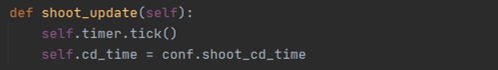
\includegraphics[width=0.5\textwidth]{Player_shoot_update}
			\caption{implementation of shoot\_update in Player}
		\end{center}
	\end{figure}
	\item[check\_shoot\_cd]
	If a player want to get the ball, the system will check if it just shoot the ball by using the timer, which begins to tick in shoot\_update.
	\begin{figure}[H]
		\begin{center}
			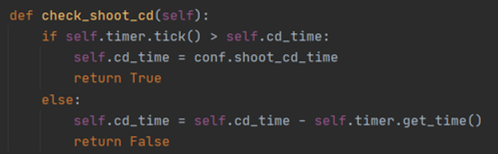
\includegraphics[width=0.7\textwidth]{Player_check_shoot_cd}
			\caption{implementation of cehck\_shoot\_cd\_time in Player}
		\end{center}
	\end{figure}
	\item[render]
	In render, the update function will be called. Then the player will be rendered through the screen, which is passed to the render method.
	\begin{figure}[H]
		\begin{center}
			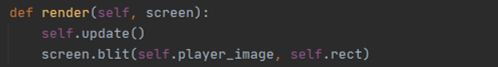
\includegraphics[width=0.5\textwidth]{Player_render}
			\caption{implementation of render in Player}
		\end{center}
	\end{figure}
\end{description}

\subsubsection{Ball}
The Ball class inherits from Sprite, which is a pre-defined class of pygame module. Below are methods of Ball.
\begin{description}
	\item[\_\_init\_\_]
	In the \_\_init\_\_ method, we define and initialize the related variavles of the ball, assign initial position to the player, and load the image of players.
	\begin{figure}[H]
		\begin{center}
			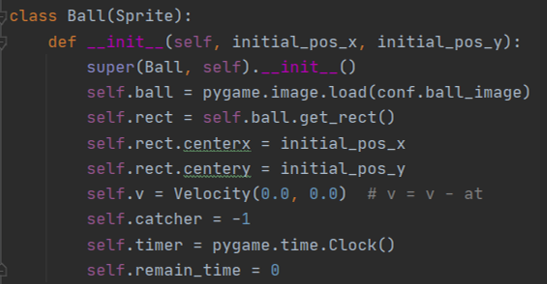
\includegraphics[width=0.7\textwidth]{Ball_init}
			\caption{implementation of \_\_init\_\_ in Ball}
		\end{center}
	\end{figure}
	\item[belong]
	In the belong, an player id is passed into this method, and it will be checked that if the ball belongs to the player with this id. 
	\begin{figure}[H]
		\begin{center}
			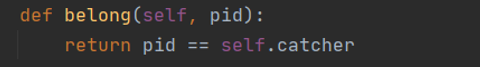
\includegraphics[width=0.5\textwidth]{Ball_belong}
			\caption{implementation of belong in Ball}
		\end{center}
	\end{figure}
	\item[caught]
	In the caught, the ball is caught by the player with given player id. And the information about tha ball would be updated.
	\begin{figure}[H]
		\begin{center}
			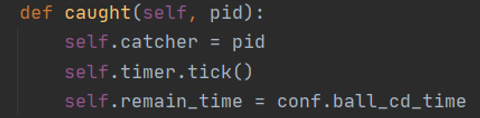
\includegraphics[width=0.5\textwidth]{Ball_caught}
			\caption{implementation of caught in Ball}
		\end{center}
	\end{figure}
	\item[copy\_pos]
	Position of ball will be updated according to the x and y value passed.
	\begin{figure}[H]
		\begin{center}
			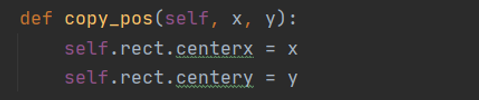
\includegraphics[width=0.5\textwidth]{Ball_copy_pos}
			\caption{implementation of copy\_pos in Ball}
		\end{center}
	\end{figure}
	\item[check\_time\_up]
	In check\_time\_up, the remain time of invincible period will be checked. If the invincible time is up, the method will return True, which means other players can steal the ball from the player catching the ball.
	\begin{figure}[H]
		\begin{center}
			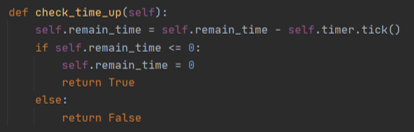
\includegraphics[width=0.7\textwidth]{Ball_check_time}
			\caption{implementation of check\_time\_up in Ball}
		\end{center}
	\end{figure}
	\item[shoot\_ball]
	Update relative information of the ball, after a player shoot the ball, and update velocity of the ball through dir\_to\_xy.
	\begin{figure}[H]
		\begin{center}
			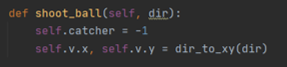
\includegraphics[width=0.5\textwidth]{Ball_shoot}
			\caption{implementation of shoot\_ball in Ball}
		\end{center}
	\end{figure}
	\begin{figure}[H]
		\begin{center}
			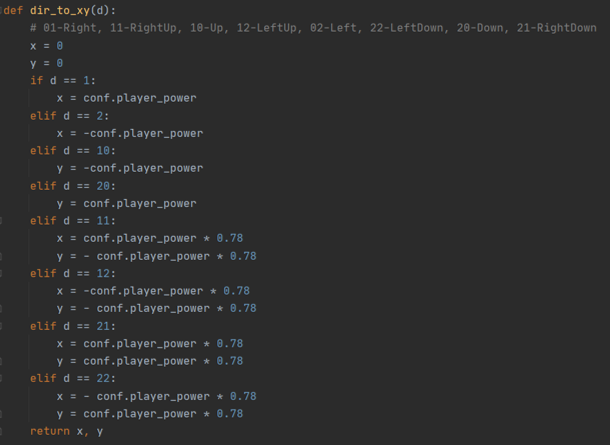
\includegraphics[width=0.9\textwidth]{dir_to_xy}
			\caption{implementation of dir\_to\_xy}
		\end{center}
	\end{figure}
	\item[update\_pos]
	In update\_pos, position of ball will be updated according to it velocity, and boundary rebounce will be done. Also, the velocity will also be updated, according to the friction of the ground through update\_v.
	\begin{figure}[H]
		\begin{center}
			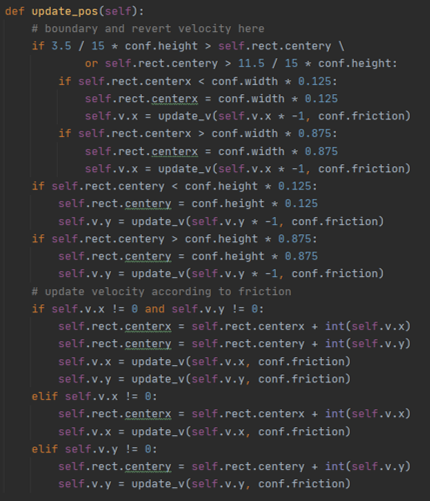
\includegraphics[width=0.9\textwidth]{Ball_update_pos}
			\caption{implementation of update\_pos in Ball}
		\end{center}
	\end{figure}
	\begin{figure}[H]
		\begin{center}
			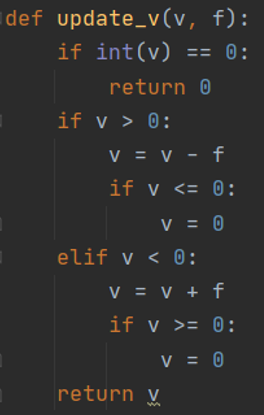
\includegraphics[width=0.3\textwidth]{update_v}
			\caption{implementation of update\_v}
		\end{center}
	\end{figure}
	\item[render]
	In render, update\_pos is called. Then, ball is rendered through the screen passed to this method.
	\begin{figure}[H]
		\begin{center}
			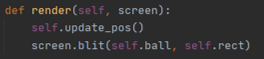
\includegraphics[width=0.5\textwidth]{Ball_render}
			\caption{implementation of render in Ball}
		\end{center}
	\end{figure}
	\item[in\_door]
	In this function, it is checked that if any team get a score. If team-0 get a score, return 0, if team-1 get a score, return 1. Otherwise, return -1.
	\begin{figure}[H]
		\begin{center}
			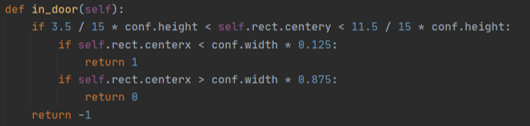
\includegraphics[width=0.9\textwidth]{Ball_in_door}
			\caption{implementation of in\_door in Ball}
		\end{center}
	\end{figure}
\end{description}

\subsubsection{Main Part}
	First, information about the game is initialized, and important variables storing information about the game are built. Here a function named initialuze\_game will be called.
	\begin{figure}[H]
	\begin{center}
		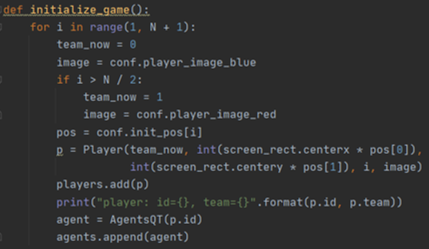
\includegraphics[width=0.9\textwidth]{initialize_game}
		\caption{implementation of initialize\_game}
	\end{center}
	\end{figure}
	In the main while loop of game execution, first each player will deal with its input passed from AI, through the relative method of Player and Ball.
	\begin{figure}[H]
	\begin{center}
		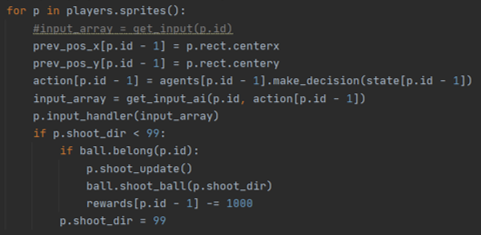
\includegraphics[width=0.9\textwidth]{deal_with_input}
		\caption{implementation of main part about dealing with input}
	\end{center}
	\end{figure}
	Then, the system will detect if there is any collision between player and ball, and judge if any player get or steal the ball according to the state of ball and the player catching the ball (if any). Then position of the ball will be updated, and sysytem will check if any team get a score. 
	\begin{figure}[H]
	\begin{center}
		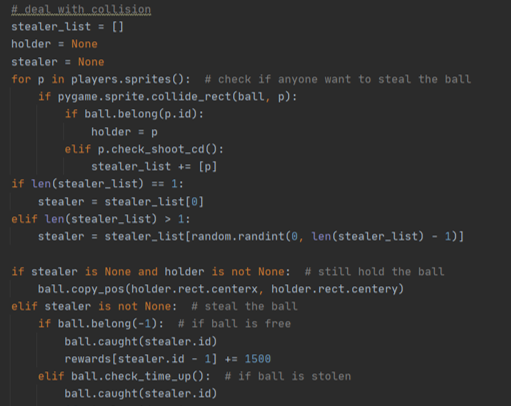
\includegraphics[width=0.9\textwidth]{collision}
		\caption{implementation of main part about collision}
	\end{center}
	\end{figure}
	Finally, iamge of every player and ball will be rendered un the screen.
	\begin{figure}[H]
		\begin{center}
			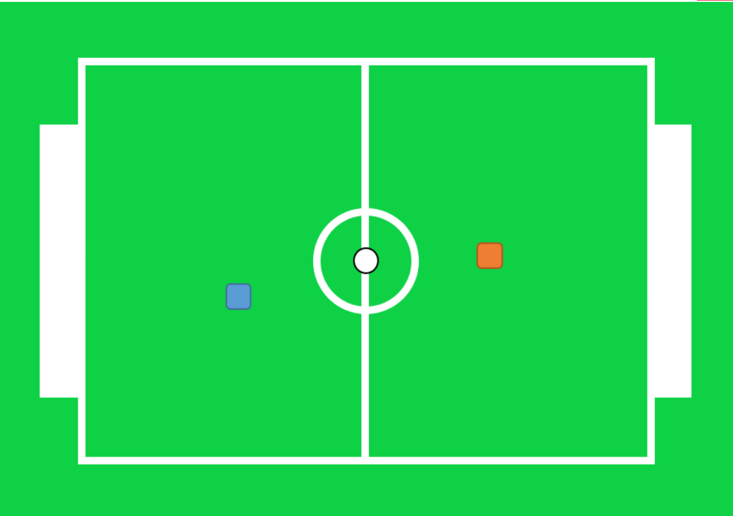
\includegraphics[width=0.9\textwidth]{game}
			\caption{Game}
		\end{center}
	\end{figure}

\subsection{AI Implementation}
	
	
%----------------------------------------------------------------------------------------
%	SECTION 6
%----------------------------------------------------------------------------------------

\section{Current Conclusion}

\begin{enumerate}
\begin{item}
The \emph{atomic weight of an element} is the relative weight of one of its atoms compared to C-12 with a weight of 12.0000000$\ldots$, hydrogen with a weight of 1.008, to oxygen with a weight of 16.00. Atomic weight is also the average weight of all the atoms of that element as they occur in nature.
\end{item}
\begin{item}
The \emph{units of atomic weight} are two-fold, with an identical numerical value. They are g/mole of atoms (or just g/mol) or amu/atom.
\end{item}
\begin{item}
\emph{Percentage discrepancy} between an accepted (literature) value and an experimental value is
\begin{equation*}
\frac{\mathrm{experimental\;result} - \mathrm{accepted\;result}}{\mathrm{accepted\;result}}
\end{equation*}
\end{item}
\end{enumerate}

%----------------------------------------------------------------------------------------
%	SECTION 5
%----------------------------------------------------------------------------------------

\section{Future Plan}

placeholder



%----------------------------------------------------------------------------------------
%	BIBLIOGRAPHY
%----------------------------------------------------------------------------------------

\begin{thebibliography}{99}
	\bibitem{ref1}Silver, David, et al. "Mastering the game of Go with deep neural networks and tree search." nature 529.7587 (2016): 484-489.
	\bibitem{ref2}Mnih, Volodymyr, et al. "Playing atari with deep reinforcement learning." arXiv preprint arXiv:1312.5602 (2013).
	\bibitem{ref3}Berner, Christopher, et al. "Dota 2 with large scale deep reinforcement learning." arXiv preprint arXiv:1912.06680 (2019).
    \bibitem{ref4}Zoph, Barret, and Quoc V. Le. "Neural architecture search with reinforcement learning." arXiv preprint arXiv:1611.01578 (2016).
    \bibitem{ref5}Mnih, Volodymyr, et al. "Human-level control through deep reinforcement learning." nature 518.7540 (2015): 529-533.
\end{thebibliography}
%----------------------------------------------------------------------------------------


\end{document}